\section{Experimental Results}
\label{sec:experimental_results}
%
We showcase our parameter optimization method for symbolic fabrics. The search space 
for the parameters is summarized in \cref{tab:search_space}.
%
\begin{table}[]
    \centering
    \begin{tabular}{c|c|c|c|c}
        Parameter & boundaries & type & distribution & manual \\
        \hline
        \baseinertia{} & $[0,1]$ & float & uniform & 0.2\\ 
        \kgeocol{} & $[0.01,1]$ & float & log & 0.03\\ 
        \kgeolimit{} & $[0.01,1]$ & float & log & 0.3\\ 
        \kgeoself{} & $[0.01,1]$ & float & log & 0.03\\ 
        \kfincol{} & $[0.01,1]$ & float & log & 0.03\\ 
        \kfinlimit{} & $[0.01,1]$ & float & log & 0.05\\ 
        \kfinself{} & $[0.01,1]$ & float & log & 0.03\\ 
        \expgeocol{} & $[1,5]$ & int & uniform & 3\\ 
        \expgeolimit{} & $[1,5]$ & int & uniform & 2\\ 
        \expgeoself{} & $[1,5]$ & int & uniform & 3\\ 
        \expfincol{} & $[1,5]$ & int & uniform & 3\\ 
        \expfinlimit{} & $[1,5]$ & int & uniform & 3\\ 
        \expfinself{} & $[1,5]$ & int & uniform & 3\\ 
        \alphab{} & $[0, 1]$ & float & uniform & 0.5\\
        \Bmin{} & $[0,1]$ & float & uniform & 0.01 \\
        \Bmax{} & $[5, 20]$ & float & uniform & 6.5 \\
        \radiusshift{} & [0.01, 0.1] & float & uniform & 0.05 \\
        \exfactor{} & [1.0, 30] & float & uniform & 15.0 \\
    \end{tabular}
    \
    \caption{Search space for parameters. Some parameters are restricted to integers, and for some
    a log-distribution is applied.}
    \label{tab:search_space}
    \vspace{-15pt}
\end{table}
%
We first analyze
the importance of tuning for optimization fabrics on the performance of trajectory
generation.
Then, we investigate
how tuned parameters can be transferred across
different robots (\cref{sub:cross_validation_robots}),
different scenarios (\cref{sub:cros_validation_tasks}),
and between simulation and real world (\cref{sub:cross_validation_transfer_real_world}).

\subsection{Experimental setup}
%
The method was tested in simulation and in the real world on a \panda{} and a
mobile manipulator composed of a \boxer{} and a \panda{}. The simulation uses
the pybullet physics engine with an interface through OpenAI-gym
\cite{spahn_urdf_environment}. 
The
different motion planning goals evaluated in this paper are: (a) reaching an
end-effector pose inside a ring of obstacles (\cref{fig:reachinginring})
(similar to the experiment in \cite{Wyk2022}) and (b) reaching an end-effector
pose above a surface with random obstacles (\cref{fig:reachingontable}). The
two scenarios will be referred to as \reachinginring{} and \reachingontable{},
see \cref{fig:tasks}. Unless stated otherwise, the weights are set to
$\weightpath=0.1, \weightcol=0.2, \weightdist=0.7$. We also use this weighted
sum as the performance metric. 
While these weights are chosen arbitrarily in this work to demonstrate
the usefulness of autotuning, they should be derived from a human evaluator
in a more realistic scenario.
We refer with \textit{manual} to an expert-tuning, see \cref{tab:search_space}
for specific parameters. During testing, the trial was randomized with changing
obstacles and goals. For autotuning on the robotic arms, we consistently used
$N=60$ trials, although the best parameter set is usually reached earlier, see
\cref{fig:history}.
%
\begin{figure}
    \centering
    \begin{subfigure}[b]{0.35\linewidth}
        \centering
        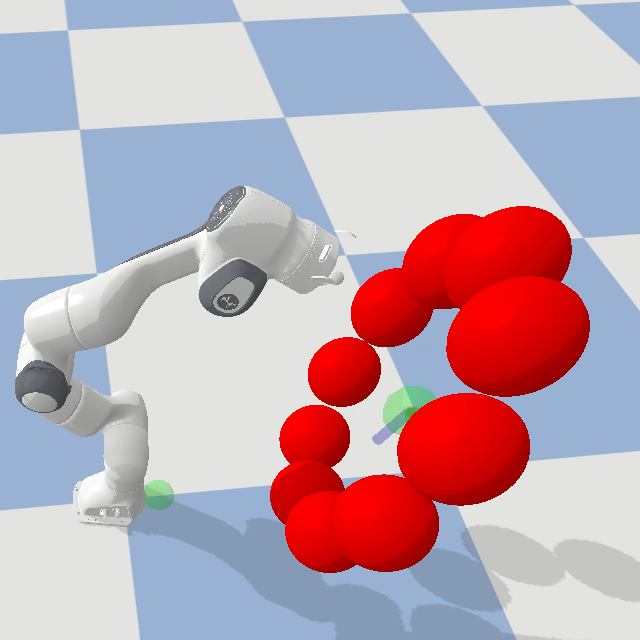
\includegraphics[width=0.8\textwidth]{task1_1.png}
        \caption{\reachinginring{}}
        \label{fig:reachinginring}
    \end{subfigure}
    \begin{subfigure}[b]{0.35\linewidth}
        \centering
        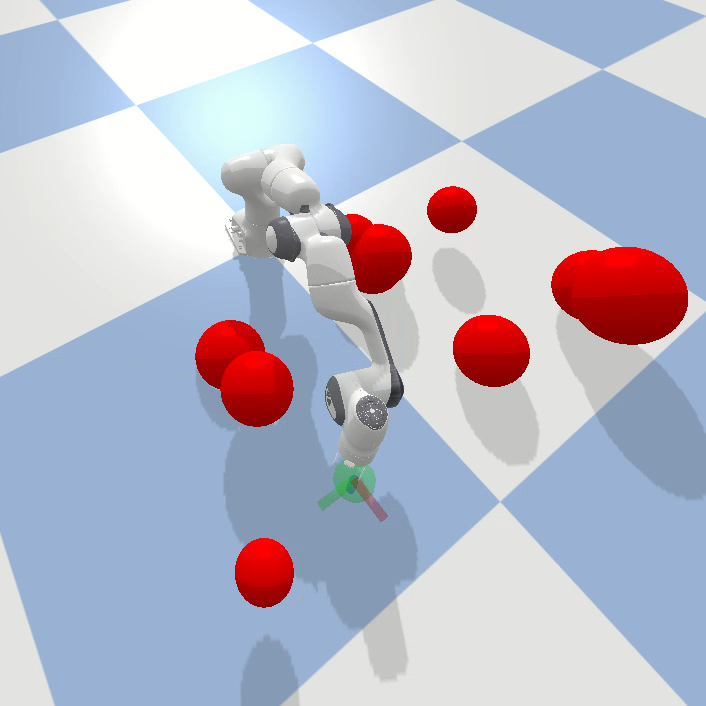
\includegraphics[width=0.8\textwidth]{task2_2.png}
        \caption{\reachingontable{}}
        \label{fig:reachingontable}
    \end{subfigure}
    \label{fig:tasks}
\end{figure}
%
\begin{figure}
    \centering
    \begin{subfigure}[b]{0.49\linewidth}
        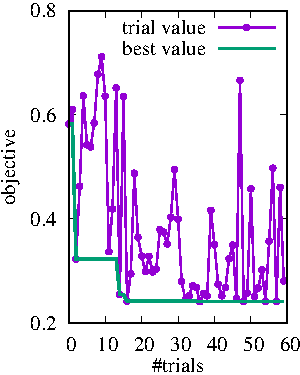
\includegraphics[width=1\textwidth]{history_panda_ring}
    \end{subfigure}
    \begin{subfigure}[b]{0.49\linewidth}
        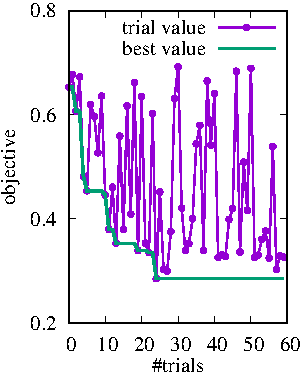
\includegraphics[width=1\textwidth]{history_panda_ring_real}
    \end{subfigure}
    \captionsetup{belowskip=-20pt}
    \caption{Optimization history for simulation (left) and real world (right) for panda robot in 
        \reachinginring{} scenario.}
    \label{fig:history}
\end{figure}

\subsection{Importance of tuning}
\label{sub:importance_tuning}
%
We compare the autotuned parameters with seven random parameter sets from the
search space and a manually tuned parameter set that we obtained through
expertise in previous works like \cite{Spahn2022}.
%
In this experiment, tuning and testing are performed on the test scenario
\reachinginring{}. Tuning is crucial for optimization
fabrics, as the performance with a random parameter set cannot compete with
tuning, \cref{fig:results_manual_random_autotune}. This result was expected and
should only demonstrate that the right parameter set is required to deploy this
method. Autotuned parameters reach a similar performance to the expert. This
result highlights the importance of tuning for optimization fabrics and shows
that autotuning is an effective way to obtain parameter sets for novice users
of optimization fabrics.
%
\begin{figure}
    \centering
    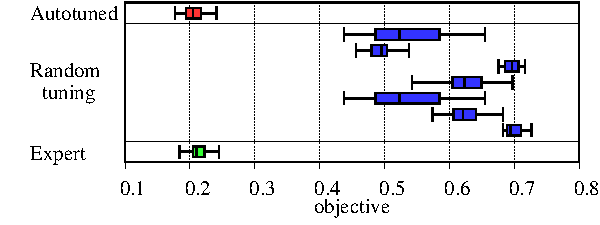
\includegraphics[width=\linewidth]{tuned_vs_random_plot}
    \caption{Evaluation for scenario \reachinginring{} autotuned parameters and compared
        to random parameter selection and manual tuning. Autotuning is able to 
        systematically outperform random parameter sets and reach expert level tuning.}
    \label{fig:results_manual_random_autotune}
\end{figure}

\begin{figure}
    \centering
    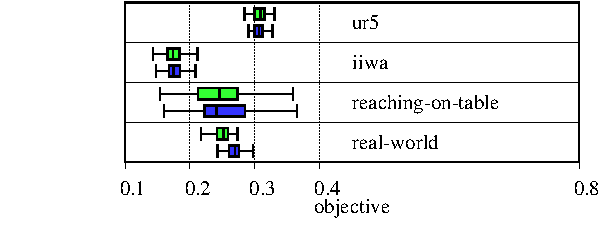
\includegraphics[width=\linewidth]{cross_validation_horizontal_plot}
    \captionsetup{belowskip=-20pt}
    \caption{
   %     Results for cross-evaluations. We evaluate the performance of
   %     the tuning with the panda robot on the \reachinginring{} case 
   %     in simulation, in the real world, and with two
   %     different robots and compare it to autotuning in the changing scenarios.
        The autotuned for the panda robot in simulation for the
        \reachinginring{} scenario on modified scenarios (blue) is compared to
        autotuned parameter sets obtained on these scenarios directly (green).
        Exchanging the robot (ur5, iiwa) and changing the scenario
        (\reachingontable{}) results in a very small loss in performance, while
        the loss is higher when parameters are transferred between simulation
        and real world (real-world).
    }
    \label{fig:cross_evaluation}
\end{figure}
%
%
\subsection{Cross validation: Transfer across robots}
\label{sub:cross_validation_robots}
%
Without any retuning, we deploy the symbolic optimization fabrics planner tuned
on the \panda{} on two other robots with similar specifications (Kuka LBR IIwa
7, Universal Robot UR5) and compare the performance with tuning performed on
the respective robot. 
Specifically, we do not change the leaf geometries and energies but change
differential maps according to relevant collision links on the robot at hand.
From \cref{fig:cross_evaluation}, we conclude that tuning is independent of the
robot. This can be explained by the fact, that optimization fabrics are a
purely geometric approach to trajectory generation and the different
dimension of the robots do not change the dynamical system enforced onto the
robot.
%
\subsection{Cross Validation: Transfer across scenarios}
\label{sub:cros_validation_tasks}
%
In the third experiment, we evaluate how well an autotuned parameter set
transfers to a different scenario. In the specific example, we use the tuning
obtained from the \reachinginring{} case and test it on \reachingontable{}.
Performance can be transferred smoothly if the objective remains the same, see
\cref{fig:cross_evaluation}. However, note that different scenario might
require generally slower motion because of a more crowded environment. Such a
step would require to retune the parameters according to the new objective.
%
\subsection{Cross Validation: Transfer real world}
\label{sub:cross_validation_transfer_real_world}
%
%
As optimization fabrics are a geometric method \cite{Wyk2022}, they should be
independent of the robot embodiment. Relying on the low-level controller. In
this paper, we investigate how the performance is affected by the transfer from
the simulation environment to the real world. 
Performance benefits from tuning in the real world highlight that low-level
controller differences affect the behavior, see \cref{fig:cross_evaluation}.
Specifically, the accumulated distance to the goal is increased ($0.14$m tuned
in the real world vs $0.16$m tuned in simulation) when tuning is transferred
between simulation and real world. Thus, there is added value in tuning in the
real world. Our framework offers to quickly tune fabrics in the real-world
using the \textit{fabrics-ros-bridge}. With relaxed performance requirements, it
is sufficient to tune in simulation.%

\subsection{Cross Validation: Transfer mobile manipulator}
%
%
Finally, we qualitatively test the performance of the tuning method on a real
mobile manipulator with 10 degrees of freedom. After only $N=30$ trials, the
robot was able to perform coupled mobile manipulation based on a visual
servoing approach \cite{chaumette2016visual}. Symbolic optimization fabrics are
especially suited for visual servoing as their symbolic character allows them
to constantly update the position of the goal. A video of this experiment is
attached to the paper.

\begin{figure}
    \centering
    \begin{subfigure}{0.5\linewidth}
        \centering
        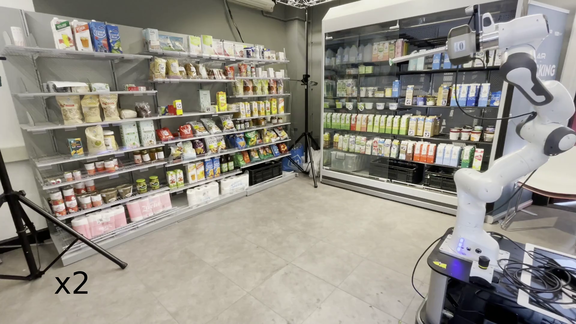
\includegraphics[width=.95\linewidth]{image_00002.png}
        \label{fig:my_label}
    \end{subfigure}%
    \begin{subfigure}{0.5\linewidth}
        \centering
        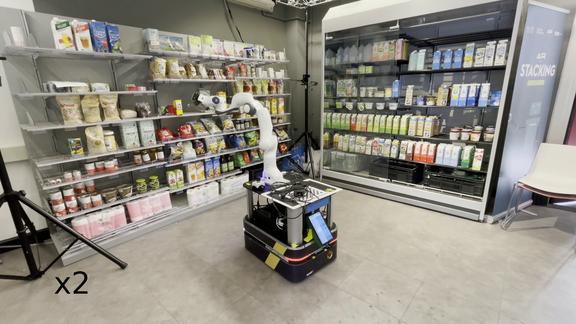
\includegraphics[width=.95\linewidth]{image_00005.png}
        \label{fig:my_label}
    \end{subfigure}
    \par\smallskip
    \begin{subfigure}{0.5\linewidth}
        \centering
        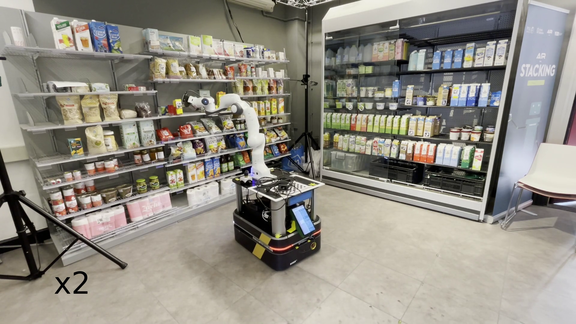
\includegraphics[width=.95\linewidth]{image_00006.png}
        \label{fig:my_label}
    \end{subfigure}%
    \begin{subfigure}{0.5\linewidth}
        \centering
        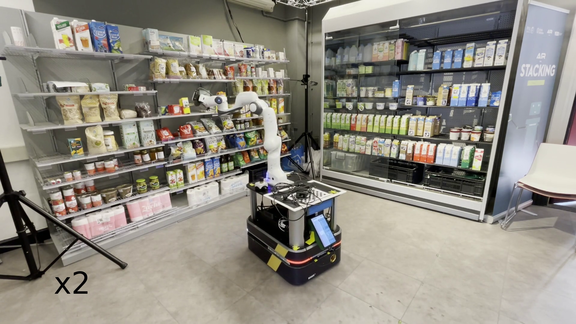
\includegraphics[width=.95\linewidth]{image_00007.png}
        \label{fig:my_label}
    \end{subfigure}%
    \captionsetup{belowskip=-10pt}
    \caption{Trajectory generation with optimization fabrics for mobile manipulator using visual serving for product picking.}
    \vspace{-10pt}
\end{figure}
%


